\documentclass[aspectratio=169]{beamer}

\usefonttheme[stillsansserifmath]{serif}
\usepackage{graphicx}
\usepackage{amsfonts}
\usepackage{mathtools, nccmath}
\usepackage{amssymb, amsmath}
\usepackage{xspace}
\usepackage{tikz}
\usepackage{standalone}
\usepackage{euler}
\usepackage{color,xcolor}
\usepackage{fontspec}
\usepackage{nameref}
\usepackage{manfnt}
\usepackage{listings}
\usepackage{xcolor}
\usepackage{algorithm}
\usepackage[noend]{algpseudocode}
\usepackage{algorithmicx}
\usepackage{docs/style}

\usepackage{xepersian}
\settextfont{Yas}

% Persian specific
\newcommand{\itmsep}[1]{\raggedleft\setlength\itemsep{#1}}
\newcommand{\itemr}{\raggedleft\setlength\itemsep{3mm}}
\newcommand{\fn}[2]{\LR{\LTRfootnote[frame,#1]{~#2}}}
%\newcommand{\fn}[2]{{\LR{\footnote[frame,#1]{{~\LR{#2}}}}}}
\newcommand{\fnn}[1]{{\LR{\footnote[frame]{{~\LR{#1}}}}}}
\newcommand{\m}[1]{\ensuremath{\mathnormal{#1}}}
\newcommand{\mc}[1]{\ensuremath{\mathtt{#1}}}
\newcommand{\scl}{\ensuremath{\Sigma^*}\xspace}
\newcommand{\gcl}{\ensuremath{\Gamma^*}\xspace}
\newcommand{\gin}{\ensuremath{\mathnormal{\in}}\xspace}
%\newcommand{\gand}{\ensuremath{\mathnormal{\land}}\xspace}
\newcommand{\gand}{\&\&\xspace}
\newcommand{\alglr}{\LTR\ttfamily\small}
\newcommand{\st}[1]{\ensuremath{\mathnormal{\{#1\}}}\xspace}
\newcommand{\gst}[1]{\ensuremath{\mathnormal{\{\text{\texttt{#1}}\}}}\xspace}
\newcommand{\cpp}{C++\xspace}
\newcommand{\enc}[1]{\ensuremath{\mathnormal{\langle#1\rangle}}\xspace}
\newcommand{\abo}[1]{\ensuremath{\mathnormal{O(#1)}}\xspace}
\newcommand{\aso}[1]{\ensuremath{\mathnormal{o(#1)}}\xspace}
\newcommand{\aom}[1]{\ensuremath{\mathnormal{\Omega(#1)}}\xspace}
\newcommand{\ath}[1]{\ensuremath{\mathnormal{\Theta(#1)}}\xspace}
\newcommand{\dom}[2]{\ensuremath{\mathnormal{\Big[ \dfrac{#1}{#2} \Big]}}\xspace}

\newcommand{\Proc}[2]{\Statex \textbf{procedure} \textsc{#1}(#2)}
\newcommand{\Func}[2]{\Statex \textbf{function} \textsc{#1}(#2)}
\newcommand{\To}{\textbf{to}\xspace}
\newcommand{\Aand}{\textbf{and}\xspace}
\newcommand{\Aor}{\textbf{or}\xspace}



\newcommand\pro{\ensuremath{\rightarrow}\xspace}
\newcommand\der{\ensuremath{\Rightarrow}\xspace}
\newcommand\ders{\ensuremath{\stackrel{\mbox{*}}{\Rightarrow}}\xspace}
\newcommand{\dern}[1]{\ensuremath{\stackrel{\mbox{\small #1}}{\Rightarrow}}\xspace}
\newcommand\move{\ensuremath{\vdash}\xspace}
\newcommand\moves{\ensuremath{\stackrel{\small *}{\vdash}}\xspace}
\newcommand{\movesn}[1]{\ensuremath{\stackrel{\small *}{\vdash_{#1}}}\xspace}
\newcommand{\moven}[1]{\ensuremath{\mathnormal{\vdash_{#1}}}\xspace}

\newcommand{\code}[1]{{\LR{\texttt{#1}}}}
\newcommand{\txtlr}[1]{\text{\LR{#1}}}


% Abbreviations
\newcommand{\ie}{\latin{i.e.,~}}
\newcommand{\eg}{\latin{e.g.,~}}
\newcommand{\cf}{\latin{cf.~}}
\newcommand{\etal}{\latin{et al.~}}
\newcommand{\etc}{\unskip~\latin{etc.}\xspace}
\newcommand{\apriori}{\latin{a priori}}
\newcommand{\wrt}{\latin{w.r.t.~}}
%\newtheorem{theorem}{Theorem}

\newcommand\NN{\ensuremath{\mathbb{N}}\xspace}
\newcommand\RR{\ensuremath{\mathbb{R}}\xspace}
\newcommand\NNS{\ensuremath{\mathbb{N}^*}\xspace}
\newcommand\NNZ{\ensuremath{\mathbb{N}\backslash\{0\}}\xspace}
\newcommand\RRP{\ensuremath{\mathbb{R}^+}\xspace}
\newcommand\vect[1]{\ensuremath{\boldsymbol{\vec{#1}}}}
\newcommand\MP{\ensuremath{\mathcal{P}}\xspace}

\newcommand\de{\mathrel{\bullet\mkern-2.5mu{\rightarrow}}}
\newcommand\ue{\mathrel{\bullet\mkern-3mu{-}\mkern-3mu\bullet}}

\DeclareMathOperator*{\argmax}{arg\,max}
\DeclareMathOperator*{\argmin}{arg\,min}

\DeclareMathOperator{\lcm}{lcm}
\DeclareMathOperator{\Spec}{Spec}
\DeclareMathOperator{\Res}{Res}
%\DeclareMathOperator{\land}{and}

\newcommand{\fl}[1]{\ensuremath{\lfloor #1 \rfloor}}
\newcommand{\bfl}[1]{\ensuremath{\big\lfloor #1 \big\rfloor}}
\newcommand{\Bfl}[1]{\ensuremath{\Big\lfloor #1 \Big\rfloor}}
\newcommand{\bgfl}[1]{\ensuremath{\bigg\lfloor #1 \bigg\rfloor}}
\newcommand{\Bgfl}[1]{\ensuremath{\Bigg\lfloor #1 \Bigg\rfloor}}

\newcommand{\cl}[1]{\ensuremath{\lceil #1 \rceil}}
\newcommand{\bcl}[1]{\ensuremath{\big\lceil #1 \big\rceil}}
\newcommand{\Bcl}[1]{\ensuremath{\Big\lceil #1 \Big\rceil}}
\newcommand{\bgcl}[1]{\ensuremath{\bigg\lceil #1 \bigg\rceil}}
\newcommand{\Bgcl}[1]{\ensuremath{\Bigg\lceil #1 \Bigg\rceil}}

\newcommand{\mtx}[1]{\begin{pmatrix} #1 \end{pmatrix}}
\newcommand{\smtx}[1]{\begin{psmallmatrix} #1 \end{psmallmatrix}}

\definecolor{commentgreen}{RGB}{2,112,10}
\definecolor{eminence}{RGB}{108,48,130}
\definecolor{brightmaroon}{rgb}{0.76, 0.13, 0.28}
\definecolor{darkred}{rgb}{0.55, 0.0, 0.0}
\lstset {
    language=C++,
    frame=tb,
    tabsize=4,
    showstringspaces=false,
    numbers=left,
    %upquote=true,
    commentstyle=\color{commentgreen},
    keywordstyle=\color{eminence},
    stringstyle=\color{darkred},
    basicstyle=\small\ttfamily, % basic font setting
    emph={int,char,double,float,unsigned,long,short,void,bool},
    emphstyle={\color{blue}},
    %escapechar=\&,
    % keyword highlighting
    %classoffset=1, % starting new class
    %otherkeywords={>,<,.,;,-,!,=,~},
    %morekeywords={>,<,.,;,-,!,=,~},
    %keywordstyle=\color{weborange},
    %classoffset=0,
}

\makeatletter
\NewDocumentCommand{\LeftComment}{s m}{%
	\IfBooleanF{#1}{\hspace*{\ALG@thistlm}}\textcolor{commentgreen}{\(~\triangleright\) #2}}
\makeatother


\newenvironment{itemframe}[2]{
\begin{frame}[environment=itemframe]{#1}

\framesubtitle{\small \color{gray} \quad #2}
\itemize
\itemr

}{
\enditemize
\end{frame}
}

\newcommand{\centerimg}[2][.5]{
    \begin{figure}[h!]
        \centering
        \includegraphics[width=#1\textwidth]{#2}
    \end{figure}
}

\usetikzlibrary{arrows,calc}
\usetikzlibrary{positioning,shapes,chains,fit}


\tikzset{
    %Define style for boxes
    node/.style={
        circle,
        draw=black, thick,
        align=center,
    },
    ss/.style={
        circle,
        draw=black,
        align=center,
    },
    proc/.style={
        rounded corners,
        draw=black,
        align=center,
    },
    ifelse/.style={
	ellipse,
	draw=black,
	align=center,
    },
    cloudy/.style={
	cloud,
	cloud puffs=12,
	cloud ignores aspect,
	align=center,
	draw=black,
    },
    txt/.style={
        draw = none,
        align = center,
        font = \footnotesize,
    },
    coin/.style={
        rectangle,
        minimum height=1mm,
        minimum width=1cm,
        draw=black,
        fill=black!20,
        rounded corners
    },
    towercolor/.style={
        fill=black!80
    },
    towerbase/.style={
        trapezium,
        trapezium angle=75,
        trapezium stretches=true,
        towercolor,
        minimum width=7mm,
        minimum height=2mm,
    },
    tower/.style={
        rectangle,
        rounded corners,
        towercolor,
        minimum width=2mm,
        minimum height=26mm,
    },
    start-end/.style={
        draw,
        rectangle,
        rounded corners,
    },
    input/.style={ % requires library shapes.geometric
        draw,
        trapezium,
        trapezium left angle=60,
        trapezium right angle=120,
    },
    operation/.style={
        draw,
        rectangle
    },
    loop/.style={ % requires library shapes.misc
        draw,
        chamfered rectangle,
        chamfered rectangle xsep=2cm
    },
    decision/.style={ % requires library shapes.geometric
        draw,
        diamond,
        aspect=#1
    },
    decision/.default=1,
    print/.style={ % requires library shapes.symbols
        draw,
        tape,
        tape bend top=none
    },
    connection/.style={
        draw,
        circle,
        radius=5pt,
    },
    process rectangle outer width/.initial=0.15cm,
    predefined process/.style={
        rectangle,
        draw,
        append after command={
        \pgfextra{
          \draw
          ($(\tikzlastnode.north west)-(0,0.5\pgflinewidth)$)--
          ($(\tikzlastnode.north west)-(\pgfkeysvalueof{/tikz/process rectangle outer width},0.5\pgflinewidth)$)--
          ($(\tikzlastnode.south west)+(-\pgfkeysvalueof{/tikz/process rectangle outer width},+0.5\pgflinewidth)$)--
          ($(\tikzlastnode.south west)+(0,0.5\pgflinewidth)$);
          \draw
          ($(\tikzlastnode.north east)-(0,0.5\pgflinewidth)$)--
          ($(\tikzlastnode.north east)+(\pgfkeysvalueof{/tikz/process rectangle outer width},-0.5\pgflinewidth)$)--
          ($(\tikzlastnode.south east)+(\pgfkeysvalueof{/tikz/process rectangle outer width},0.5\pgflinewidth)$)--
          ($(\tikzlastnode.south east)+(0,0.5\pgflinewidth)$);
        }  
        },
        text width=#1,
        align=center
    },
    predefined process/.default=1.75cm,
    man op/.style={ % requires library shapes.geometric
        draw,
        trapezium,
        shape border rotate=180,
        text width=2cm,
        align=center,
    },
    extract/.style={
        draw,
        isosceles triangle,
        isosceles triangle apex angle=60,
        shape border rotate=90
    },
    merge/.style={
        draw,
        isosceles triangle,
        isosceles triangle apex angle=60,
        shape border rotate=-90
    },
}


\title{طراحی الگوریتم‌ها}
\author{
آرش شفیعی
}

\institute{
\\

\includegraphics[height=1.2cm]{logos/ui.png}
%\\
%دانشگاه اصفهان
}
\date{}

\begin{document}

\begin{frame}[plain]
\begin{center}
به نام خدا
\end{center}

\maketitle

%\begin{center}
%{\footnotesize arash.shafiei@gmail.com}
%\end{center}

\end{frame}
\setcounter{framenumber}{0}

%\input{docs/licence}

\raggedleft

%%%%%%%%%%%%
%\begin{frame}{فهرست مطالب}
%\begin{flushright}
%  \tableofcontents
%\end{flushright}
%\end{frame}
%%%%%%%%%%%%

%%%%%%%%%%%%
\section{الگوریتم‌های پیشرفته در گراف}
%------------------------------------------------------------------------
\begin{frame}{يادآوری}
	\begin{itemize}\itemr
		\item[-]
کتاب CLRS که مرجع اصلی این درس است دو تعریف مجزا برای گراف ارائه می‌دهد:
\item[۱]
گراف بدون جهت: این گراف نمی‌تواند طوقه یا یال موازی داشته باشد.
\item[۲]
گراف جهت دار: این گراف می‌تواند طوقه داشته باشد اما نمی‌تواند یال موازی داشته باشد. البته دو یال می‌تواند بین دو راس یکسان وجود داشته باشد به شرطی جهت آنها مخالف یکدیگر باشد. برای مثال شکل زیر یک گراف فاقد یال موازی است.

\begin{figure}[h!]
\centering
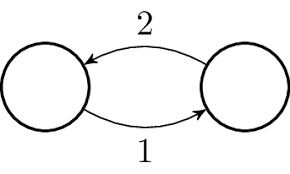
\includegraphics[width=0.2\textwidth]{figs/chap01/1.png}
\end{figure}
\item[-]
در هر یک از مسائل بسته به ذات مسئله نوع خاصی از گراف به عنوان ورودی در نظر گرفته می‌شود. برای مثال ورودی مسئله کوتاه ترین مسیر در حالت کلی یک گراف جهت دار و وزن دار است.
\end{itemize}
\end{frame}


%------------------------------------------------------------------------
\begin{frame}{يادآوری}
	\begin{itemize}\itemr
\item[-]
الگوریتم‌های گراف برخلاف بیشتر الگوریتم‌هایدارای دو متغییر تاثیر گذار در اندازه ورودی‌اند: تعداد یال‌ها (|E|) و تعداد رئوس (|V|) .
\item[-]
بر اساس قرارداد کتاب CLRS می‌توان در نمادهای مجانبی از قرار دادن نماد اندازه در اطراف V و E صرف‌نظر ‌کرد.

\item[-]
الگوریتم‌های گراف به طور معمول در دو حالت بررسی می‌شوند:
\item[الف]
زمانی که گراف متراکم باشد: در این حالت فرض میکنیم همه رئوس به هم متصل هستند بنابراین تعداد یال ها از مرتبه
\ath{V^2}
است.
\item[ب]
زمانی که گراف خلوت باشد:‌ در این حالت به طور معمول فرض می‌شود که تعداد یال‌ها از مرتبه
\ath{V}
است.

	\end{itemize}
\end{frame}

%------------------------------------------------------------------------
\begin{frame}{يادآوری}
\begin{itemize}\itemr
\item[-]
پیچیدگی زمانی ارائه شده برای یک الگوریتم گراف را می‌توان در دو حالت بالا تحلیل کرد. برای مثال تمرین زیر از کتاب CLRS را در نظر بگیرید:

\begin{figure}[h!]
\centering
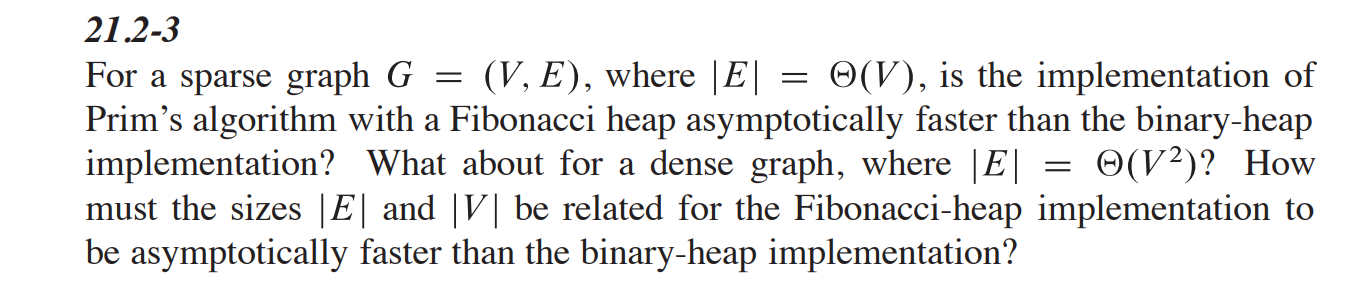
\includegraphics[width=\textwidth]{figs/chap01/2.png}
\end{figure}

\end{itemize}
\end{frame}

%------------------------------------------------------------------------
\begin{frame}{يادآوری}
\begin{itemize}\itemr
\item[-]
پیچیدگی زمانی الگوریتم پریم با استفاده از هرم دودویی از مرتبه
\m{O(E logV+V lgV)}
و با استفاده از هرم فیبوناچی از مرتبه
\m{O(E+V logV)}
است. با جایگذاری V به جای E در این دو تابع درمی‌یابیم که در گراف خلوت هر دو پیاده‌سازی‌ از لحاظ مجانبی سرعت یکسانی دارند و از مرتبه
\m{O(Vlg V)}
اند. اما در گراف متراکم پیاده‌سازی با هرم فیبوناچی از لحاظ مجانبی سریع تر و از مرتبه
\m{O(lgV^2)}
 است.
\item[-]
چنین تحلیلی در دیگر الگوریتم‌‌های گراف هم کاربرد دارد. برای مثال الگوریتم فلوید-وارشال از مرتبه زمانی
\m{O(V^3)}
 است. از تحلیل این تابع می‌توان نتیجه گرفت خلوت یا متراکم بودن گراف از نظر مجانبی تاثیری بر سرعت این الگوریتم ندارد.
\end{itemize}
\end{frame}




%------------------------------------------------------------------------
\begin{frame}{الگوریتم جانسون}
\begin{itemize}\itemr
\item[-]
الگوریتم جانسون
\fn{1}{Johnson Algorithm}
مانند الگوریتم فلوید وارشال برای یافتن کوتاه ترین مسیر بین هر دو راس گراف است. این الگوریتم برای گراف‌های خلوت پبچیدگی زمانی کمتری نسبت به بقیه روش‌ها (فلوید وارشال و روش شبیه‌سازی ضرب ماترسی) دارد.

\item[-]
الگوریتم جانسون -مانند الگوریتم بلمن فورد- می‌تواند روی گراف دارای یال منفی کوتاه ترین مسیر را به درستی محاسبه کند و وجود دور منفی در گراف را تشخیص و گزارش دهد. (گراف دارای دور منفی در مسئله کوتاه ترین مسیر یک حالت خطا محسوب می‌شود.)
\footnote{برای گراف دارای دور منفی یافتن کوتاه ترین مسیر ساده می‌تواند کاربرد داشته‌باشد. این مسئله ان‌پی-سخت است.}
\end{itemize}
\end{frame}

%------------------------------------------------------------------------
\begin{frame}{الگوریتم جانسون}
	\begin{itemize}\itemr
\item[-]
برای طراحی یک الگوریتم مسئله کوتاه‌ترین مسیر بین هر جفت رأس می‌توان V بار اجرا کردن یکی از الگوریتم‌های کوتاه‌ترین مسیرهای هم مبداء را به عنوان یک حد بالا برای مرتبه زمانی تحلیل کرد.

\item[-]
برای مثال
\m{|V|}
بار اجرای الگوریتم بلمن فورد مرتبه
\m{O(V^2E)}
و
\m{|V|}
بار اجرای الگوریتم دایجسترا مرتبه
\m{O(VE+V^2lgV)}
را به دست می‌دهد.
\item[-]
روش دوم سریع‌تر است امّا در گراف‌‌هایی که یال منفی داشته باشند به درستی کار نمی‌کند.
	\end{itemize}
\end{frame}

%------------------------------------------------------------------------
\begin{frame}{الگوریتم جانسون}
\begin{itemize}\itemr
\item[-]
الگوریتم جانسون نیز از ایده‌ایی مشابه استفاده می‌کند. این الگوریتم هر دو الگوریتم بلمن-فورد و دایجسترا را فراخوانی می‌کند؛
\item[۱]
جانسون در مرحله اول، الگوریتم بلمن-فورد را استفاده می‌کند تا وجود دور منفی را تشخیص دهد و در صورتی که دور منفی وجود داشت آن را گزارش داده و کار تمام می‌شود.
\item[۲]
در صورتی که دور منفی وجود نداشت، این الگوریتم با استفاده از روشی که در ادامه بررسی خواهد شد، همه وزن‌ها را به مقادیر غیر منفی نگاشت می‌کند.
\item[۳]
حال که همه وزن‌‌های غیر منفی شده‌اند برای هر رأس یک بار الگوریتم دایجسترا اجرا می‌شود تا کوتاه ترین مسیرها از هر رأس به بقیه رئوس محاسبه شوند.
\end{itemize}
\end{frame}

%------------------------------------------------------------------------
\begin{frame}{الگوریتم جانسون}
	\begin{itemize}\itemr
\item[-]
اما چطور باید وزن‌های گراف را به مقادیر غیر منفی نگاشت کرد؟ واضح است که بعد از تغییر وزن‌ها نباید کوتاه ترین مسیرها را تغییر کنند. برای مثال اضافه کردن یک مقدار ثابت به همه وزن‌ها نگاشت مناسبی نیست. برای درک بهتر این موضوع به مثال زیر توجه کنید:
\begin{center}
	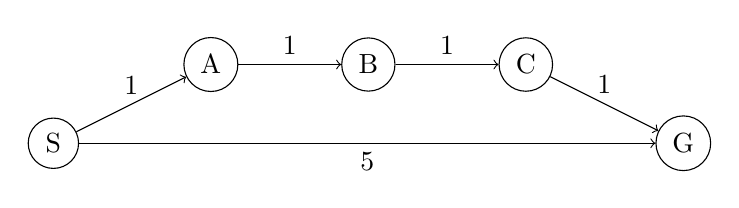
\begin{tikzpicture}[->]
		\node[circle,draw] (S) at (0,0) {S};
		\node[circle,draw] (G) at (8,0) {G};
		\node[circle,draw] (A) at (2,1) {A};
		\node[circle,draw] (B) at (4,1) {B};
		\node[circle,draw] (C) at (6,1) {C};

		\draw (S) -- node[below] {5} (G);
		\draw (S) -- node[above] {1} (A);
		\draw (A) -- node[above] {1} (B);
		\draw (B) -- node[above] {1} (C);
		\draw (C) -- node[above] {1} (G);
	\end{tikzpicture}
\end{center}
\item[-]
اضافه کردن یک واحد به همه یال‌ها کوتاه ترین مسیر از S به G را تغییر می‌دهد:

\begin{center}
	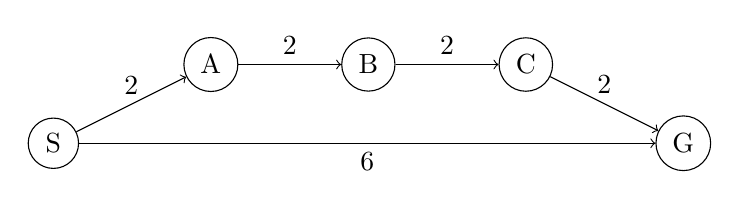
\begin{tikzpicture}[->]
		\node[circle,draw] (S) at (0,0) {S};
		\node[circle,draw] (G) at (8,0) {G};
		\node[circle,draw] (A) at (2,1) {A};
		\node[circle,draw] (B) at (4,1) {B};
		\node[circle,draw] (C) at (6,1) {C};

		\draw (S) -- node[below] {6} (G);
		\draw (S) -- node[above] {2} (A);
		\draw (A) -- node[above] {2} (B);
		\draw (B) -- node[above] {2} (C);
		\draw (C) -- node[above] {2} (G);
	\end{tikzpicture}
\end{center}

	\end{itemize}
\end{frame}

%------------------------------------------------------------------------
\begin{frame}{الگوریتم جانسون}
	\begin{itemize}\itemr
\item[-]
بیایید ویژگی‌های این تغییر وزن را به طور دقیق‌تر بررسی کنیم؛\\
فرض کنید وزن‌های گراف توسط تابعی به نام «تابع وزن»
\fn{1}{weight function}
داده شده. به طوری که وزن یال بین u و v برابر است با
\m{w(u, v)}.
آنگاه تابع وزن جدیدی مانند
\m{\hat{w}}
باید این دو ویژگی را داشته باشد:
\item[1]
به ازای هر
\m{u, v \in E}
مسیری مانند p با استفاده از تابع وزن
\m{w}
یک کوتاه ترین مسیر از u به v است اگر و تنها اگر مسیر p با استفاده از تابع وزن
\m{\hat{w}}
نیز یک کوتاه ترین مسیر باشد.
\item[2]
به ازای هر
\m{u, v \in E}
مقدار
\m{\hat{w}(u, v)}
غیر منفی باشد.
	\end{itemize}
\end{frame}

%------------------------------------------------------------------------
\begin{frame}{الگوریتم جانسون}
	\begin{itemize}\itemr
\item[-]
الگوریتم جانسون از این تغییر وزن استفاده می‌کند:
\begin{align*}
	\m{\hat{w}(u, v)} = \m{w(u, v)} + h(u) - h(v)
\end{align*}
\item[-]
به طوری که u رأس شروع و v رأس پایان یال است و h تابعی است که به هر رأس یک عدد حقیقی نسبت می‌دهد.
\item[-]
در ادامه ثابت خواهیم کرد که این تغییر وزن به ازای هر تابع h کوتاه‌ترین مسیرها را تغییر نمی‌دهد اما برای تبدیل همه وزن‌ها به مقادیر غیر منفی، تابع h باید به درستی تعریف شود.
	\end{itemize}
\end{frame}
%------------------------------------------------------------------------
\begin{frame}{الگوریتم جانسون}
	\begin{itemize}\itemr
		\item[-]
ابتدا باید ثابت ‌کنیم رابطه تغییر وزن ارائه شده ویژگی اول را ارضاء می‌کند.
		\item
فرض کنید
		\m{ p= \langle v_0, v_1, ..., v_k \rangle}
یک مسیر از
		\m{v_0}
به
		\m{v_k}
باشد. همچنین وزن کل مسیر p با تابع وزن w را با  w(p) نشان می‌دهیم. آنگاه
		\m{\hat{w}}
برابر است با:
		\begin{align*}
			\m{\hat{w}(p)= (\hat{w}(v_0, v_1) + h(v_0) -  h(v_1)) + (\hat{w}(v_1, v_2) + h(v_1) -  h(v_2)) + }
			\\
			\m{(\hat{w}(v_2, v_3) + h(v_2) -  h(v_3)) + ... + (\hat{w}(v_{k-1}, v_k) + h(v_{k-1}) -  h(v_k))}
		\end{align*}

	\end{itemize}
\end{frame}
%------------------------------------------------------------------------
\begin{frame}{الگوریتم جانسون}
	\begin{itemize}\itemr
\item
رابطه بالا نشان می‌دهد برای هر رأس مثل u، مقدار h(u) به وزن یک یال اضافه می‌شود و از یال بعدی کسر می‌شود (به غیر از رأس ابتدا و انتهای مسیر). بعد از ساده‌سازی به این رابطه می‌رسیم:
\begin{align*}
	\m{\hat{w}(p)=w(p) + h(h(v_0) - h(v_k)}
\end{align*}
\item
بنابراین برای هر دو رأس مشخص به همه کوتاه‌ترین مسیرهای بین آن دو رأس یک مقدار ثابت اضافه می‌شود پس این نگاشت وزن کوتاه ترین مسیرها را تغییر نمی‌دهد.
	\end{itemize}
\end{frame}

%------------------------------------------------------------------------
\begin{frame}{الگوریتم جانسون}
	\begin{itemize}\itemr
		\item[-]
هدف بعدی این است که شرایطی فراهم کنیم که ویژگی دوم هم برقرار باشد. برای این کار یک رأس جدید به نام s به گراف اضافه می‌کنیم. سپس این رأس را با یال‌هایی با وزن صفر به همه رئوس دیگر متصل می‌کنیم به طوری که یال ‌ها از s خارج شوند.
		\begin{figure}[h!]
			\centering
			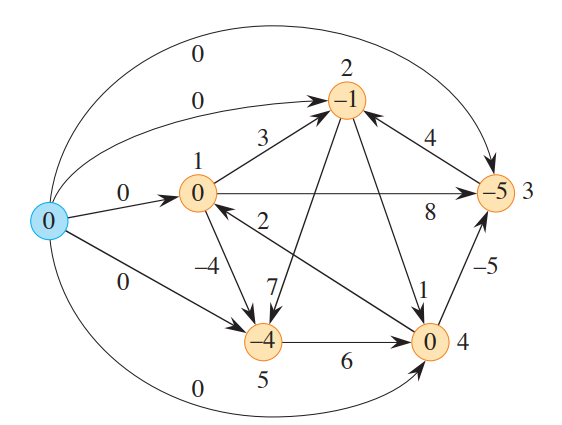
\includegraphics[width=.4\textwidth]{figs/chap02/4.png}
		\end{figure}
شکل بالا نمونه‌ایی از این تغییر را نشان می‌دهد (رأس آبی رنگ به گراف اضافه شده‌است).
	\end{itemize}
\end{frame}

%------------------------------------------------------------------------
\begin{frame}{الگوریتم جانسون}
	\begin{itemize}\itemr
		\item
سپس تعریف می‌کنیم مقدار h برای هر رأس مثل v برابر است با کوتاه ترین مسیر از s به v . در شکل بالا نیز اعداد نوشته‌شده بر رأس‌ها به همین طریق محاسبه شده‌اند.
		\item
حال با استفاده از نامساوی مثلثاتی می‌دانیم که به ازای هر
		\m{(u, v \in E)}
رابطه زیر برقرار است:
		\begin{center}
			\m{h(v) \leqslant h(u)+w(u, v) } \\

		\end{center}
		\item
اگر رابطه بالا برقرار نباشد نتیجه می‌شود که مسیر h(v) کوتاه‌ترین مسیر نبوده و به تناقض می‌رسیم.
		\item
سپس h(u) را به سمت راست نامساوی می‌بریم:
		\begin{center}
			\m{0\leqslant w(u, v) + h(u) - h(v)}
		\end{center}
		\item
سمت راست این نامساوی همان رابطه‌ایی است که برای $\hat{w}$ تعریف شد. بنابراین ثابت شد که به ازای هر
		\m{(u, v \in E)}
مقدار $\hat{w}$ غیر منفی است.
	\end{itemize}
\end{frame}

%------------------------------------------------------------------------
\begin{frame}{الگوریتم جانسون}
	\begin{itemize}\itemr
		\item[-]
درستی الگوریتم جانسون ثابت شد. شکل زیر یک نمونه از گراف تغییر وزن یافته توسط الگوریتم جانسون است:
		\begin{figure}[h!]
			\centering
			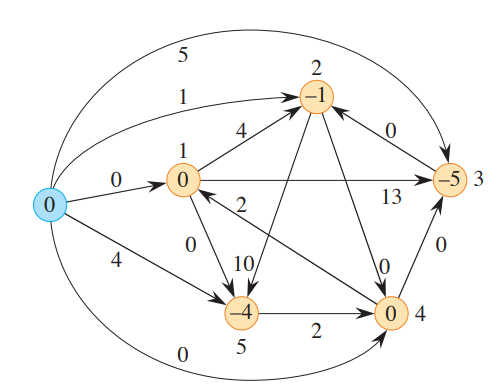
\includegraphics[width=.3\textwidth]{figs/chap02/5.png}
		\end{figure}

		\item[-]
قبلا اشاره شد که الگوریتم جانسون از الگوریتم بلمن-فورد برای تشخیص دور منفی استفاده می‌کند. همچنین دیدم که برای محاسبه تابع h نیاز به مقادیر کوتاه‌ترین مسیر از s به بقیه رئوس نیاز داریم. می‌دانیم الگوریتم بلمن-فورد توانایی محاسبه هر دوی این موارد را دارد. بنابراین الگوریتم جانسون با یک بار اجرای بلمن-فورد هم کوتاه‌ترین مسیرها از s را محاسبه می‌کند و هم وجود دور منفی را تشخیص می‌دهد.

	\end{itemize}
\end{frame}

%------------------------------------------------------------------------
\begin{frame}{الگوریتم جانسون}
	\begin{itemize}\itemr
		\item[-]
		برای یافتن وزن اصلی یک مسیر از رابطه زیر استفاده می‌کنیم:
		\begin{center}
			\m{w(p(u, v)) = \hat{w}(p(u, v)) + h(v) - h(u) }
		\end{center}

		\item[-]
		در نهایت به تحیلی پیچیدگی زمانی الگوریتم جانسون می‌پردازیم:
		\item
		اجرای $|V|$ بار الگوریتم دایجسترا زمان‌برترین مرحله الگوریتم جانسون است بنابراین -مانند دایجسترا- باید گراف را در لیست مجاورتی ذخیره کنیم. حال اگر فرض کنیم الگوریتم دایجسترا با استفاده از هرم فیبوناچی پیاده‌سازی شده‌است، پیچیدگی زمانی برابر است با
		\m{O(V^2lgV+VE)}
		که از ضرب یک
		\m{|V|}
		در مرتبه زمانی دایجسترا به دست آمده‌است.
		\item
		در صورتی که گراف خلوت باشد مرتبه زمانی این الگوریتم برابر است
		\m{O(V^2lgV)}.
		در حالی که الگوریتم فلوید-وارشال برای گراف خلوت از مربته زمانی
		\m{O(V^3)}
		است.

	\end{itemize}
\end{frame}


%%%%%%%%%%%%

%%%%%%%%%%%%
%\section*{References}
%\begin{frame}<0>[noframenumbering]
%\bibliographystyle{apalike}
%\bibliography{docs/bib}
%\end{frame}
%%%%%%%%%%%%

\end{document}
